\section{Experimental Evaluation}\label{sec:results}

\subsection{Experimental Setup}
\label{sec:expSetup}

All GPU kernels used to evaluate S-L1 were executed on an Nvidia GeForce GTX Titan Black GPU connected to 6GB of GPU memory with a total of 2,880 computing cores running at 980MHz.
As described in Section~\ref{GPUBackground}, the GTX Titan Black is from the Kepler family and has 15 streaming
multiprocessors (SMXs), each with 192 computing cores,  and 64KB of on-chip memory (of which 48KB is assigned to shared memory).

All GPU-based applications were implemented in CUDA, using CUDA toolkit and GPU driver release 7.0.28 installed on a 64-bit Ubuntu 14.04 Linux with kernel 3.16.0-33.
All applications are compiled with the corresponding version of the {\it nvcc} compiler using optimization level three.

For each experiment, we ran the target application using different thread configurations,
and only considered the configuration with the best execution time for reporting and comparison purposes.\footnote{ 
    GPGPU programmers typically experimentally run their applications  with different thread configurations to
    determine the optimal number of threads and from then on run that configuration.}
Specifically, we tested each application using 512 different thread configurations,
starting with 15 blocks of 128 threads (for a total of 1,920 threads) and increased the number of threads in 128 increments, up to 480 blocks of 1,024 threads (for a total of 480K threads).

\begin{table*}[ht]
{
\begin{center}
%{\tiny
\resizebox{16cm}{1.9cm}
{
  \begin{tabular}{|p{2.8cm}|p{14.4cm}|p{3.5cm}|} \hline
         {\bf Application} & {\bf Description} &  {\bf Used number of data structures}\\
\hline
	  {Upper} &   {Converts all text in an input document from lowercase to uppercase.} &  {2}\\  \hline
	  {WC} &   {Counts the number of words and lines in an input document.} &  {1}\\ \hline
	  {DNA Assembly} & {merges fragments of a DNA sequence to reconstruct a larger sequence~\cite{dnaassembly}.} & {3}\\ \hline
	  {Opinion Finder} & {analyzes the sentiments of tweets associated with a given subject (i.e. a set of given keywords)~\cite{wilson2005opinionfinder}} &  {4}\\ \hline
	  {Inverted Index} & {Builds reverse index from a series of HTML files.} & {3}\\ \hline
	  {Page View Count} & {Counts the number of hits of each URL in a web log.} & {3}\\ \hline
          {MasterCard Affinity} & {finds all merchants that are frequently visited by customers of a target merchant X~\cite{mokhtari2014bigkernel}} & {3}\\ \hline
	  {Matrix Multiply} & {Calculates the multiplication of two input matrices. This is a naive version and does not use shared memory.} & {3}\\ \hline
	  {Grep} & {Finds the string matching a given pattern and outputs the line containing that string.} & {2 (1 in shared memory)}\\ \hline
	  {Kmeans} & {Partitions $n$ particles into $k$ clusters so that particles are assigned to the cluster with the nearest mean.} & {2 (1 in shared memory)}\\ \hline
  \end{tabular}
}
%}
\end{center}
}
\vspace{-0.1cm}
\caption{\footnotesize\textnormal{Ten streaming applications used in our experimental performance evaluation
and the number of data structures they use in their main loop. S-L1 determines the number of data
structures to cache at runtime, which could vary from run to run depending on the available size of shared memory per
thread (see Section~\ref{sec:overview}).}} %title of the table
\label{tab:apps}
\vspace{-0.0cm}
\end{table*}

\subsection{S-L1 performance evaluation for GPU-local applications}
\label{sec:perfevaluation}

\begin{figure}[t]
\center
\includegraphics[scale=0.7]{1speedups.eps}
\vspace{-0.0cm}
\caption{\footnotesize\textnormal{Speedup when using S-L1 relative to no L1 caching.}}
\label{fig:perfbenefit}
\end{figure}
\vspace{-0.0cm}

\begin{figure}[t]
\center
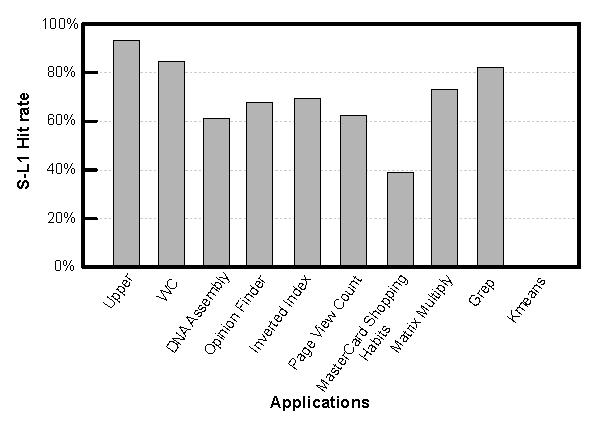
\includegraphics[scale=0.9]{3memoryAcceessReuction.eps}
\vspace{-0.0cm}
\caption{\footnotesize\textnormal{S-L1 hit rate.}}
\label{fig:sl1hitrate}
\end{figure}
%\vspace{-0.2cm}


We applied S-L1 to the ten streaming applications listed in Table~\ref{tab:apps}. 
There is no standard benchmark suite for GPU streaming applications, so we selected 6 representative applications, 2 simple scientific applications (\texttt{MatrixMultiply} and \texttt{Kmeans}), and 2 extreme applications to stress test S-L1: \texttt{wc}, which has minimal computation (only counter increments) for each character access, and \texttt{upper}, which is similar to \texttt{wc} but may modify the characters.
For each experiment, the data accessed by the applications is already located in GPU memory.


Figure~\ref{fig:perfbenefit} shows the performance of our 10 benchmark streaming applications when run with S-L1 and hardware L1 
relative to the performance of the same applications run with no L1 caching (L2 cache is enabled in all cases).
On average, the applications using S-L1 run 1.9 times faster than when they use the hardware L1 and 2.1 times faster than when
run with no L1 caching.

With hardware L1, performance improves to at most 35\% and in some cases degrades significantly.
In particular, \texttt{wc},  \texttt{PageViewCount}, and \texttt{Matrix
Multiply} exhibit slowdown.
We attribute the poor performance to the extra DRAM transactions due to the
constant thrashing of L1 cache lines: each cache miss results in four DRAM
transactions (four 32-byte transactions to fill the 128-byte cache line), three
transactions more than what is actually required to fulfill the requesting
memory access instruction, a phenomenon originally observed by by Jia et al.~\cite{jia2012characterizing}.



With S-L1, some applications (e.g., \texttt{upper} and \texttt{wc}) run
multiple times faster than with hardware L1, while other applications (e.g., \texttt{grep}
and \texttt{Kmeans}) experience slight slowdowns. The benefits obtained from
S-L1 depends on a number of factors.
First, the attained cache hit rate obviously has a large effect.
Figure~\ref{fig:sl1hitrate} depicts the S-L1 hit rate for all benchmarks. 
Overall, the hit rate is quite high, in part because most of the applications have high spatial
locality (which is to be expected for streaming applications). 
As an extreme example, consider \texttt{wc}, where each thread accesses a sequence of adjacent characters, so each S-L1 miss is typically followed by 15 hits, given a 16 byte cache line.
Kmeans is an exception: because the application allocates much of the shared memory for its own purposes, there is insufficient space for S-L1 cache lines, and hence the effective S-L1 hit rate is zero for this application.\footnote{
	Because Kmeans allocates space in shared memory dynamically at run time,
	the compiler cannot know that there is not enough space for S-L1  cache lines ---
	otherwise it potentially could have avoided adding the code required for S-L1. In
	practice, Kmeans would be run without S-L1, so it would not have to incur the S-L1 overheads.}

A second factor is the memory intensity of the applications; i.e., the ratio of memory access instructions to the total number of instructions executed.
Some applications (e.g., \texttt{upper} and \texttt{wc}) are memory bound and hence benefit from S-L1.
At the other extreme, \texttt{grep} doesn't perform as well despite having a
high cache hit rate, mainly because it becomes instruction throughput bound
after applying S-L1 due to its recursive algorithm. The benefits of the
caching layer is negated by the extra instructions that need to be executed
because of the software implementation of S-L1.



\begin{figure}[t]
\center
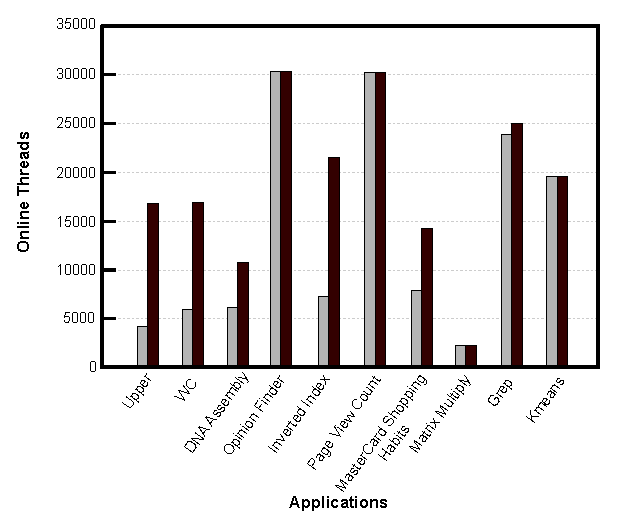
\includegraphics[scale=0.75]{8higherParallelism.eps}
\vspace{-0.0cm}
\caption{\footnotesize\textnormal{The optimal number of online threads (that leads to the best execution times) with and without S-L1.}}
\label{fig:levelprallelism}
\end{figure}
%\vspace{-0.2cm}

%\begin{figure}[t]
%\center
%\includegraphics[scale=0.89]{10L2HitRateWC.eps}
%\vspace{-0.0cm}
%\caption{\footnotesize\textnormal{L2 hit rate for \texttt{wc}.}}
%\label{fig:l2hitrate}
%\end{figure}
%\vspace{-0.2cm}

A third factor is the degree to which S-L1 enables extra productive thread parallelism, thus improving GPU core utilization.
Figure~\ref{fig:levelprallelism} shows the number of \emph{online} threads\footnote{
    I.e., threads that run at the same time on all multiprocessors, the maximum of which can be 30K threads on our GPU.}
that result in the best performance for each application with S-L1 and with hardware L1.
Overall, applications perform best with a large number of threads when using S-L1 compared to hardware L1,
because hardware L1 leads to increased L1 and L2 cache thrashing. 

%An example of the L2 cache thrashing when L1 is enalbed is
%is shown in Figure~\ref{fig:l2hitrate}, which shows the L2 cache hit rate of \texttt{wc} as a function of the number of
%threads per SMX, when the cache hit rate drops to around 10\% at 1,024 threads.


%For example, Figure~\ref{fig:l2hitrate} shows the L2 cache hit rate of \texttt{wc} as a function of
%the number of threads per SMX, where the cache hit rate drops to around 10\% at 1,024 threads.

%Compared to S-L1, the benefit of hardware L1 cache is rather limited (shown in Figure~\ref{fig:perfbenefit}). Overall, the performance gains with the L1 are limited to under 35\%
%and in some cases result in slowdowns. In particular, \texttt{wc},  \texttt{PageViewCount}, and \texttt{Matrix Multiply} exhibit slowdown when L1 is enabled.
%We attribute this to the extra DRAM transactions that are resulted from constant thrashing of L1 cache.
%Note that, when L1 is enalbed, each cache miss results in four DRAM transactions (four 32-byte transactions to fill a 128-byte L1 cache line), three transactions more than
%what actually is required to fulfill the requesting memory access instruction.
%This phenomenon was originally observed by by Jia et al.~\cite{jia2012characterizing}.
%Two further interesting observations are worth noting. First, unlike S-L1, hardware L1 improves the performance of \texttt{grep} reasonably well.
%We attribute this to the fact that the hardware L1 incurs no extra instruction overhead, which for \texttt{grep} is significant because it is already computationally intensive. 


\subsection{Evaluation of S-L1 for data residing in CPU memory}

\begin{figure}[t]
\center
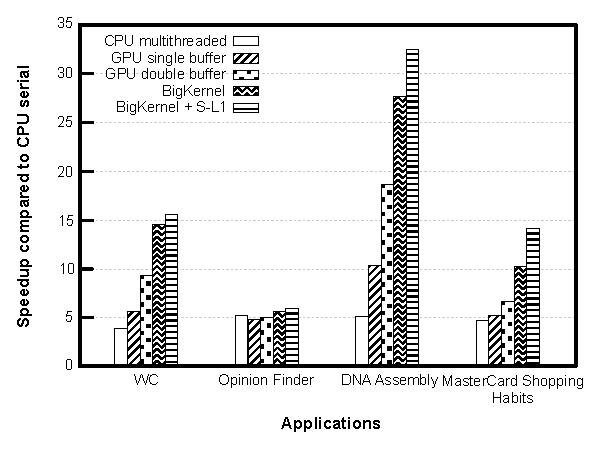
\includegraphics[scale=0.80]{11bigkernelAndSl1.eps}
\vspace{-0.0cm}
\caption{\footnotesize\textnormal{Speedup of four GPU applications processing large data sets located in CPU memory relative to the CPU serial versions.}}
\label{fig:bigkernelandsl1}
\end{figure}
%\vspace{-0.2cm}


For big data-style applications, the data will not fit in GPU memory because of the limited memory size. Hence, in this
subsection, we consider the performance of four applications with data sets large enough to not fit in GPU memory. We
ran these applications under five different scenarios:
\begin{enumerate}
\item CPU multithreaded when run on a 3.7GHz Intel Core i7-4820K with 24GB of dual-channel memory clocked at 1.8 GHz;
\item GPU using a single buffer to transfer data between CPU and GPU;
\item GPU using state-of-the-art double buffering to transfer data between CPU and GPU;
\item GPU using BigKernel~\cite{mokhtari2014bigkernel}; and
\item GPU using BigKernel combined with S-L1.
\end{enumerate} 
We selected to combine S-L1 with BigKernel in particular, because BigKernel is,
to the best of our knowledge,
the currently best performing system for data intensive GPU streaming
applications~\cite{mokhtari2014bigkernel}.

Figure~\ref{fig:bigkernelandsl1} shows the results.
For all four applications, using BigKernel with S-L1 performs the best,
and for all but one application the performance is an order of magnitude better than the multithreaded CPU version.
Compared to BigKernel alone, BigKernel with S-L1 is 1.19X faster.
Limits in thread parallelism is the primary reason BigKernel is prevented from performing better when combined with
S-L1, because BigKernel requires the use of many registers.\footnote{When a kernel uses high number of registers, an SMX
will schedule fewer {\it online threads} to be able to provide them with the required number of registers.} As shown in
Figure~\ref{fig:levelprallelism}, one of the ways S-L1 improves performance is by allowing applications to efficiently
exploit higher degrees of parallelism.

%Low parallelism can limit
%the performance gain of a potentially improved memory sub-system. 
%is that adding S-L1 to BigKernel increases register pressure, which often prevents the program t

%often leading to register spillage, in
%part because BigKernel itself already uses many registers.
%We are still working on optimizing this.
%\todo{Can we provide any more detail here? Seems to be hand waving... What "proof" can we give?}

%\todo{Note, I don't buy your second reason, and I don't think you have evidence to back it up, so I cut  it.}
% First, since the memory accesses of BigKernel implementations are already
% coalesced, they often exhibit reasonable performance, leaving a rather small room for 
% improvement by S-L1.

%\begin{figure}[t]
%\center
%\includegraphics[scale=0.23]{5hardwareL1Benefit.png}
%\vspace{-0.2cm}
%\caption{\footnotesize\textnormal{Speedup obtained when using the hardware L1 cache on the older GTX 560.}}
%\label{fig:l1hitrate}
%\end{figure}
%\vspace{-0.2cm}



\subsection{S-L1 overheads}
\label{sec:sl1overheadsresults}

\begin{figure}[t]
\center
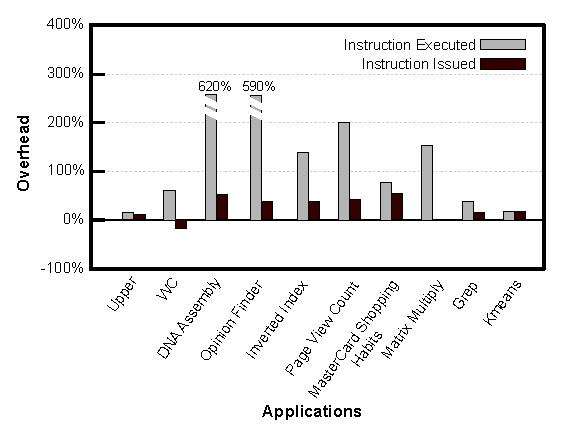
\includegraphics[scale=0.93]{4instructionIssueOverhead.eps}
\vspace{-0.0cm}
\caption{\footnotesize\textnormal{Extra instructions executed and issued (in \%) due to S-L1.}}
\label{fig:instexecissuedoverhead}
\end{figure}
%\vspace{-0.2cm}

S-L1 has significant overhead because it is implemented in software. 
However, based on our experiments, the monitoring phase accounts for less than 1\% of this overhead.
A minimum of 4 and potentially well over 100 extra
instructions are executed for each memory access.
Figure~\ref{fig:instexecissuedoverhead} depicts the increase in the number of instructions, both executed and issued,
when using S-L1 compared to when using hardware L1.
Executed instructions are the total number of instructions completed, while 
issued instructions also count the times an instruction is ``replayed'' because it
encountered a long latency event such as a memory load.

The increase in the number of executed instructions is significant: 220\% on average. 
The reason is obvious: each memory access instruction is transformed to additionally call a function that needs to be executed. 
On the other hand, the increase in the number of issued instructions is more reasonable: 25\% on average. 
(For \texttt{wc} and \texttt{MatrixMultiply} the number of issued instructions actually decreases.)
The reason issued instructions increase less than executed instructions is that S-L1 provides for improved memory performance, which reduces the number of required 
instruction replays.


\begin{figure}[t]
\center
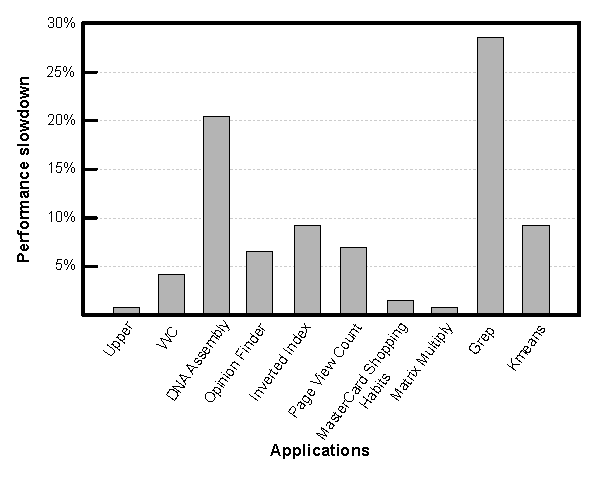
\includegraphics[scale=0.82]{7cachingOverhead.eps}
\vspace{-0.0cm}
\caption{\footnotesize\textnormal{Overhead of S-L1 when it is enabled but not used to cache data.}}
\label{fig:sl1overhead}
\end{figure}



To evaluate S-L1 overheads when accessing non-cached data structures, we ran our benchmarks with S-L1 enabled but all
data structures marked as non-cacheable. Figure~\ref{fig:sl1overhead} shows that the overhead is 8\% on average.
The primary source of the overhead is attributed to executing the memory access function that is called for each memory access.
As suggested in Section~\ref{sec:perfevaluation}, one potential way to avoid this overhead is have the compiler not
transform memory accesses to data structures that are found not worthy of caching -- e.g. a data
structure that is statically known not exhibit any caching benefit.

%introduces for data structures that are not cached, we ran our benchmarks with S-L1, but with all data structures marked as non-cacheable.
%Figure~\ref{fig:sl1overhead} shows the overhead incurred in this case: 8\% on average.
%Based on our experiments, the monitoring phase accounts for less than 1\% of this overhead. 
%The rest of the overhead is attributed to executing the memory access function that is called for each memory access.


\subsection{Effect of S-L1 cache line size}
\label{sec:cachelineeffect}


\begin{figure}[t]
\center
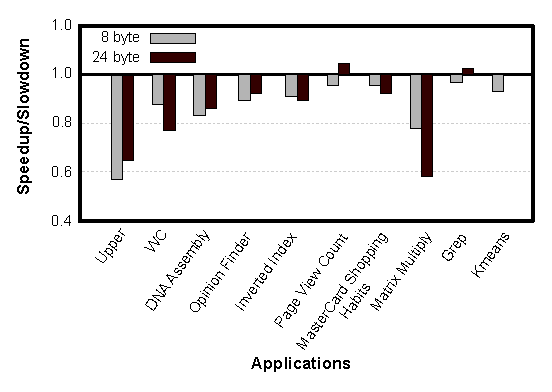
\includegraphics[scale=0.88]{6differentCachelineSizes.eps}
\vspace{-0.0cm}
\caption{\footnotesize\textnormal{Slowdown/speedup when using 8B and 24B cache lines over using 16B cache lines.}}
\label{fig:cachelinesize}
\end{figure}
%\vspace{-0.2cm}

Figure~\ref{fig:cachelinesize} compares the overall performance of applications when using different variations of S-L1 using different cache line sizes. 
Specifically, we show the performance improvement/loss for 8-byte and 24-byte cache lines over
16-byte cache lines.\footnote{We did not choose 32 as a potential cache line size since it is more
than the size of shared memory that will be assigned to a threads, if SMXs are fully occupied (i.e.
2048 threads), given the maximum size of shared memory (i.e. 48KB).}
%\todo{Say why 24B (as opposed to 32B)?}

In most cases, 16-byte cache lines seems to be best choice. 
As we described in Section~\ref{sec:overview}, we believe this is mainly because 16-bytes is the widest available load/store size on GPU ISA and hence, the entire cache line can be read/written with one memory access.

Decreasing the cache line size to 8-bytes impacts performance negatively in every case, since the cache then typically needs to execute the inserted memory access function twice as often for a fixed amount of streaming data to be processed by the application. 
Note that our benchmarks primarily consist of streaming applications that have high spatial locality and that consume most of the data in a cache lines.

Increasing the cache line size to 24-bytes also reduces performance in all but two cases, mainly
because 24 bytes do not provide much additional benefit over 16 bytes, yet require two memory accesses to fill a cache line instead of one.
For example to process 48 characters accessed sequentially, a 16B cache line results in 3 misses and thus 3 L2/DRAM accesses, whereas a 24B cache line results in 2 misses and thus 4 L2/DRAM accesses.




